\documentclass{article}
\usepackage[margin=1in]{geometry} 
\usepackage{amsmath,amsthm,amssymb,amsfonts, fancyhdr, color, comment, graphicx, environ}
\usepackage{fancyhdr}
\usepackage{extramarks}
\usepackage{amsmath}
\usepackage{amsthm}
\usepackage{amsfonts}
\usepackage{tikz}
\usepackage[plain]{algorithm}
\usepackage{algpseudocode}
\usepackage{xcolor}
\usepackage{mdframed}
%\usepackage{indentfirst}
\usepackage[shortlabels]{enumitem}
\usepackage{hyperref}
\usepackage{blindtext}
%\renewcommand{\footrulewidth}{0.8 pt}
\hypersetup{
    colorlinks=true,
    linkcolor=blue,
    filecolor=magenta,      
    urlcolor=blue,
}

\DeclareMathOperator*{\argmax}{arg\,max}
\DeclareMathOperator*{\argmin}{arg\,min}

\usepackage{float}

\usepackage{minted}

\setminted{
    linenos=true
}

%\pagestyle{fancy}
\usepackage{parskip}

\usepackage{caption}
\captionsetup[figure]{font = sl}

%\lhead{\group}
%\rhead{\firstxmark} 
%\chead{\textbf{}}
%\lfoot{Prof. Lorenzo Masia}
%\rfoot{Universität Heidelberg}

%\newenvironment{problem}[2][Problem]
%    { \begin{mdframed}[backgroundcolor=gray!20] \textbf{#1 #2} \\}
%    {  \end{mdframed}}
%\newenvironment{solution}{\textbf{Solution}}

\newcommand{\enterProblemHeader}[1]{
    \nobreak\extramarks{#1}{}\nobreak{}
}
%\newcounter{ProblemCounter}
%\setcounter{ProblemCounter}{1}

\usepackage{biblatex} %Imports biblatex package
\addbibresource{bibliography.bib} %Import the bibliography file


\begin{document}
\title{\bf\huge Solving Bomberman \\ with Q-table and Neural Networks \\[0.5em] \normalfont \Large Machine Learning Essentials (Summer 2023)
        }

\author{\Large Group: \textbf{Demolitionist} \hspace{-0.5em}\raisebox{-.65em}{\includegraphics[height=2em]{bomb.png}} \large \vspace{1em}\\\makebox[10em][r]{Behrooz Montazeran}\hspace{1em}\makebox[10em][l]{3769073}\\ \makebox[10em][r]{Jannis Heising}\hspace{1em}\makebox[10em][l]{4028349}\\[0.2em] \makebox[10em][r]{Tomáš Sláma}\hspace{1em}\makebox[10em][l]{3768224}}
\date{\large \today}

\makeatletter
    \begin{titlepage}
        \begin{center}
	   { \includegraphics[width=7cm]{avatar.png}}
	   {\ \\ \ \\}
        \vbox{}\vspace{1cm}
            {\@title }\\[4cm]%
            {\@author}\\[2.5cm]%
            {\large Instructor: \bf Prof. Ullrich Köthe\\ \ \\}
            \vfill\hfill {\@date\\}

        \end{center}
    \end{titlepage}
\makeatother


\tableofcontents

\clearpage

%%%%%%%%%%%%%%%%%%%%%%%%%%%%%%%%%%%%%%%%%%%%%%%%%%%%%%%%%%%%%%%%%%%%%%%%%%%%%%%%%%%%%%%%%%%%%%%%%%%%%%%%%%%%%%%%%%%%%%%%%%%

\section{Introduction}

\subsection[Problem Statement]{{Problem Statement}\normalsize \normalfont \it \hfill Jannis}

The goal of this project was to develop an artificial intelligence which employs machine learning techniques to master a simplified version of the classical game Bomberman. The game consists of a grid-shaped playing field containing evenly-spaced walls and populated with crates, some of which contain coins, on which up to four agents compete to score the most points, see Figure~\ref{fig:bomberman-startpos}. Collecting a coin is worth one point and killing another agent is worth five points. In order to kill an opponent or destroy a crate to potentially reveal the coin within, the agents can place bombs at their current location, after which they should move out of its blast radius before it explodes.

\begin{figure}[h]
    \centering
    \includegraphics[width=.6\linewidth]{figures/bomberman_startpos.png}
    %\caption{An example of the game in action. The four agents are depicted as robot heads with different colors. On the left, a coin has been revealed by blowing up a crate. On the right, a bomb has just exploded, and the smoke indicates that this area is still deadly.}
    \caption{The starting position of a round. The four agents are depicted as robot heads with different colors.}
    \label{fig:bomberman-startpos}
\end{figure}

The game advances in discrete time steps. In each step, an agent can choose to perform one of six actions: move up, right, down, or left, place a bomb, or do nothing. Each grid position can only be inhabited by at most one object, meaning that agents are obstructed by bombs and other agents. In each round there are nine coins to be collected. A round ends after 400 time steps or if only one agent remains, all crates are destroyed, all coins are collected and no bombs are present.

\subsection[Game Difficulty and Feature Selection]{{Game Difficulty and Feature Selection}\normalsize \normalfont \it \hfill Jannis}

Before designing an agent, one should gauge the skill ceiling of the game. This helps to make an informed decision on what aspects of the game the agent should know about. If the game turns out to be rather trivial, then even a small amount of information about the current game state might suffice to make the best decision.

\clearpage

First of all, consider the simple case of two agents competing on a playing field without any crates. Because only one bomb per agent can be present at any time, it is easy to see that neither agent can kill the other, assuming both play adequately. Thus, in order to secure a kill in a real game, the agent has to use the environment to their advantage, be it crates forming a dead end or other agents blocking the escape path. This requires at least a moderate level of awareness of the agent's surroundings.\par

As a second example, consider Figure~\ref{fig:bomberman-example}. The pink agent has wound up in quite a predicament: it has been cornered by the green agent and is completely paralyzed. Its only valid actions are waiting and placing a bomb. Luckily, the green agent cannot place a bomb until its current one has exploded, so the pink agent might have a chance to survive. Clearly, if it waits forever, it will be killed, so the question is when to place a bomb. Suicide might be an acceptable outcome if pink already has a winning score, but since the game has only just commenced, this is unlikely. It turns out that green can always block the escape path, assuming perfect play. So, perhaps the most sensible strategy would be to place a bomb immediately in the hopes of spooking green into running away and freeing pink. In fact, waiting around might not be in green's best interest as it gives yellow and blue time to collect coins.\par

\begin{figure}[h]
    \centering
    \includegraphics[width=.6\linewidth]{figures/bomberman_example.png}
    \caption{An example of the game in action. Can pink survive?}
    \label{fig:bomberman-example}
\end{figure}

The example illustrates that a perfect agent might need a lot of information: Its immediate surroundings, bomb fuse timers, the scoreboard, perhaps even the entire playing field in order to estimate the opponents' winning chances. However, an agent taking many inputs is harder to train than one taking a few hand-picked features. Due to the time constraints of the project, it is advisable to lean towards a small number of features that convey information about the agent's immediate surroundings. The agent will not play perfectly, but should achieve decent performance after only a few hours or days of training.

\clearpage

\subsection[Available Methods]{{Available Methods}\normalsize \normalfont \it \hfill Jannis}

The problem at hand can be classified as model-free reinforcement learning. Problems of this type are usually approached with some variant of Q-learning, where a so-called \textit{action-value function} $Q$ is trained to associate a given state and an action to be performed in that state with an estimate of the reward which the agent is expected to achieve in the future after performing that action. As explained above, our agent does not know the entire game state but only a few derived features, so $Q$ takes these features instead of the state as input.\par
Apart from feature selection, Q-learning variants mostly differ in the function class from which $Q$ is selected, for example:

\begin{itemize}
    \item \textbf{Q-table:} Simply storing a value for each input is the most straight-forward approach. In theory, any function can be perfectly represented in this way. In practice, however, memory-size contingencies arise when the feature space is too large. Moreover, this approach is unable to generalize; different states must be trained separately, no matter how similar they are, and states that are not encountered during training are an enigma to the agent.
    
    \item \textbf{Neural network:} Being universal function approximators and having easy-to-use python libraries makes neural networks a standard approach. If the layer sizes are chosen appropriately, neural networks excel at generalizing. For training, one typically uses gradient descent. Note that neural networks are particularly suited to be used with the full game state instead of hand-crafted features; one speaks of a \textit{deep Q-network} (DQN). In this case, the first few network layers are interpreted as ``learned features".

    \item \textbf{Regression forest:} An ensemble method of relatively primitive building blocks, regression forests aim to employ a sort of ``wisdom of the crowd" by, for example, training decision trees on different parts of the training data and averaging their responses. One possible training method is to replace the worst-performing tree with a newly trained one in each step.
\end{itemize}

Additionally, there are different possibilities to arrive at the desired Q-value after having performed an action and having been rewarded for it:

\begin{itemize}
    \item \textbf{State-action-reward-state-action (SARSA)}: The Q-value is updated based on the reward $R_{t}$ and the estimated reward granted for the proceeding action. The update formula reads:
    \begin{align*}
        Y_t &:= R_t + \gamma \cdot Q(s_{t+1}, a_{t+1}),\\
        Q(s_t, a_t) &:= Q(s_t, a_t) + \mu \cdot \left(Y_t - Q(s_t, a_t)\right).
    \end{align*}

    \item \textbf{Temporal difference (TD)}: Similar to SARSA, but instead of using the $Q$-value of the concrete action taken in step $t+1$, one uses the best possible $Q$-value in state $s_{t+1}$ (based on the current approximation):
    \begin{align*}
        Y_t &:= R_t + \gamma \cdot \max_a Q(s_{t+1}, a),\\
        Q(s_t, a_t) &:= Q(s_t, a_t) + \mu \cdot \left(Y_t - Q(s_t, a_t)\right).
    \end{align*}

    \item \textbf{n-step TD:} As a generalization of plain TD, one can improve the estimation by taking rewards which lie further into the future into account:
    \begin{align*}
        Y_t &:= \sum_{t' = t}^{t+n-1} \gamma^{t'-t} R_{t'} + \gamma^n \cdot \max_a Q(s_{t+n}, a),\\
        Q(s_t, a_t) &:= Q(s_t, a_t) + \mu \cdot \left(Y_t - Q(s_t, a_t)\right).
    \end{align*}
\end{itemize}

To improve stability of the training process, the function $Q$ may be duplicated into a \textit{policy model}, which is responsible for performing actions, and a \textit{target model}, which is trained on the results of these actions. The policy model is then either slowly updated over time to resemble the target model or completely replaced by it periodically.

\clearpage

Finally, one can choose different update strategies:

\begin{itemize}
    \item \textbf{Online learning:} A training step is applied after each time step.
    \item \textbf{Episodic learning:} One or more training steps are applied after each episode, i.e. game round.
    \item \textbf{Offline learning:} Training is done sporadically; States and actions are recorded to be used as a large training set.
\end{itemize}

\subsection[Development Outline]{{Development Outline}\normalsize \normalfont \it \hfill Jannis}

The project code can be found in our \href{https://github.com/xiaoxiae/BombermanML}{GitHub Repository}.\par

For our two main approaches, we decided to use a Q-table (implemented as \texttt{q\_agent}) and a neural network (\texttt{binary\_agent}). The main challenge was coming up with an appropriate amount of features to balance the aforementioned trade-off between agent awareness and trainability. Additionally, we tested a more complex set of features on which to train the neural network (\texttt{distance\_agent}), with moderate success. All our methods use one-step TD and online learning. The neural network approaches additionally keep a policy model.

\subsection[Progress Tracking]{{Progress Tracking}\normalsize \normalfont \it \hfill Jannis}

While training a model, it is vital to keep track of its skill level. To this end, we implemented an elo rating system~\cite{wiki:elo}. As a first step, we calculated a rating for the four agents provided for comparison, namely \texttt{coin\_collector\_agent}, \texttt{peaceful\_agent}, \texttt{random\_agent}, and \texttt{rule\_based\_agent}. The agents started with a rating of 1000. Each pair of agents competed for 100 rounds, after which their elo rating was determined with the following update formula:

\begin{minted}{python}
expected_result = 1 / (10 ** ((b - a) / 400) + 1)
difference = k * (actual_result - expected_result)

a += difference
b -= difference
\end{minted}

Here, \textit{a} and \textit{b} are the ratings of two competing agents A and B, \textit{k} is the co-called \textit{K-factor} which regulates how fast ratings can change, and \texttt{actual\_result} is the result of a given round, where a value of $1$ indicates a win for agent A, $0.5$ a draw, and $0$ a win for agent B. Thus, a good agent stands to gain less from a victory against a bad agent than it might lose after a defeat in the same match-up.\par
%Because only four agents are competing in this first step, the rating can fluctuate a lot depending on the order in which the rounds were played. Hence, we run the elo calculation several times with shuffled results to achieve a more stable result and to gauge the fluctuation. Our results were the following:
Because the rating can fluctuate a lot depending on the order in which the rounds were played, we run the elo calculation with the same games several times ($1\,000$ by default) with shuffled results to achieve a more stable result and to gauge the fluctuation. Our results were the following:

\begin{center}
\begin{tabular}{rrcr}
\textbf{rule\_based\_agent} & 1508 & \hspace{-.8em}±\hspace{-.8em} & 20.0 \\
\textbf{coin\_collector\_agent} & 1426 & \hspace{-.8em}±\hspace{-.8em} & 20.0 \\
\textbf{random\_agent} & 533 & \hspace{-.8em}±\hspace{-.8em} & 2.8 \\
\textbf{peaceful\_agent} & 531 & \hspace{-.8em}±\hspace{-.8em} & 3.0
\end{tabular}
\end{center}

These values then served as a basis for an elo estimation of our trained agents. To keep a consistent baseline, the ratings of the four base agents were not updated in subsequent matches against new agents.\par
Because elo calculation for new agents requires at least 400 rounds to be played (possibly more, depending on how many custom agents were added), we additionally implemented a faster but less thorough option to estimate an agent's skill level: In \textit{duel} mode, the selected agent plays 50 rounds against \texttt{rule\_based\_agent}, the results of which directly serve as the evaluation.

\clearpage

\section[Methods]{{Methods}\normalsize \normalfont \it \hfill Behrooz}

In this section two methods that were employed by our team is clarified. First Q-table as a simple method of reinforcement learning and then Q-learning with neural network. 

\subsection[Q-table]{{Q-table}}
\subsubsection[Construction of Q-table]{Construction of Q-table{\normalsize \normalfont \it \hfill Behrooz}}

Q-Table or simply lookup table \cite{Reinforecement-Learning} is where the maximum expected future rewards for action at each state are calculated. Basically, this table will guide the agent to the best action at each state. Columns consists of actions and the rows are built by states. Each Q-table score "Q-value" will be the maximum expected future reward that the agent will get if it takes that action at that state. This is an iterative process, as is needed to improve the Q-Table at each iteration.


 In the deployment of Q-table in bomberman game actions are\textbf{(UP, RIGHT, DOWN, LEFT, WAIT, BOMB)} and states are feature vectors extracted from the game. The first construction of the early idea of the lookup table is depicted below:
 

\begin{figure}[h]
    \centering
    \includegraphics[width=.8\linewidth]{figures/q-table/q-table.pdf}
    \caption{Sample Q-table with one sample state, relative actions and respective Q-values}
    \label{fig:early-q-table}
\end{figure}



In the bomberman game, finding the best possible and smallest vector features, which would be lately converted to state-action pairs in the Q-table is the most challenging part of construction, which was acquired by the following process:

The Q-table of the first q-agent is constructed by using linked dictionaries, in which the first keys are concatenation of agent's current position to the binary vector of the nearest items to it. The second keys or the keys of inner dictionary is the action list, which would be valued by the respective Q-values during training. To initialize such a Q-table, a list of keys from the position cell of free tiles (all tiles except walls that are always fixed) containing \textbf{\textit{16 × 16 – 49 = 207}} free positions cell is made, which is then concatenated to a list of all combination of (0, 1) in a vector with 10 elements,\{\textit{see Figure:}\ref{fig:initialized-q-table}\}. Finally this linked dictionary is initialized with zero values.

\begin{figure}[h]
    \centering
    \includegraphics[width=.8\linewidth]{figures/q-table/linked-dict.pdf}
    \caption{Initialized linked dictionary with zero values }
    \label{fig:linked-dict}
\end{figure}




As it is shown in the \{\textit{Figure:}\ref{fig:initialized-q-table}\}, the list of features consists of the following:

\begin{itemize}
    \item index of outer key $0$: \textbf{current position} of the agent
    \item index of outer key $1 \ldots \phantom{0}5$: direction to the nearest \textbf{coin} or \textbf{safety} 
    \item index of outer key $6 \ldots 10$: direction to the nearest \textbf{crate} or where placing a bomb will \textbf{possibly kill a player}
\end{itemize}




However, this idea failed very soon as the agent was indifferent against any changes to the reward's values. Nevertheless, this implementation of Q-table lighted the path to the number of states that the agent might encounter during the game. Theoretically there should be a maximum of $\textbf{\textit{207}} \times {2^{10}} \times \textbf{\textit{6 = 1,271,808}}$ possible states, in which there are maximum 207 free positions tiles for the agent to go, maximum 1024 possible actions-state according to the nearest items and maximum 6 actions that would be valued during training, nevertheless, after ten thousands of rounds the agent learned just a few states (less than two hundred). This small number of states brought the idea of a bigger feature vector that can differentiate variant directions to the different items.Therefore, the feature vector of length 22 elements was aimed with the following structure:


\begin{figure}[h]
    \centering
    \includegraphics[width=.8\linewidth]{figures/q-table/initialized-q-table.pdf}
    \caption{Illustration of outer keys in initialized Q-table with zero values }
    \label{fig:initialized-q-table}
\end{figure}


\begin{itemize}
    \item index of outer key $\phantom{0}0 \ldots \phantom{0}4$: direction to the nearest \textbf{coin}
    \item index of outer key $\phantom{0}5 \ldots \phantom{0}9$: direction to the nearest \textbf{crate} 
    \item index of outer key $10 \ldots 14$: direction to the where placing a bomb will \textbf{possibly kill a player}
    \item index of outer key $15 \ldots 19$: direction to \textbf{safety} (if in danger of dying)
    \item index of outer key $20$: \textbf{can place a bomb} and there is a way to escape it
    \item index of outer key $21$: \textbf{current position} of the agent
\end{itemize}


Again the above structure of the vector was a combination of binary items and a tuple of current position of the agent. Nevertheless, the problem of learning did not resolved until the length of feature vector reduced to 21 elements (without the current position of the agent). In designing the q-agent-v1 this feature vector is used, but initializing such a huge dictionary caused big problems and above all of them memory-space limitation. Therefore, the idea of this agent and the next versions was to let the agent go with completely random actions to discover the world and ,therefore, new states, which is completely described in \textit{training q-agent} section. The finalized structure of features and the Q-table is depicted in \{\textit{Figure:}\ref{fig:final-q-table}\}. 



\begin{figure}[h]
    \centering
    \includegraphics[width=.8\linewidth]{figures/q-table/final-q-table.pdf}
    \caption{The finalized structure of the Q-table with a sample state and sample Q-values. }
    \label{fig:final-q-table}
\end{figure}

In the sample state above the direction to the nearest coin is from the left, the nearest crates is placed on downward, there is no path to any enemies and the agent has the capability of using bomb. From the respective Q-values and according to epsilon policy that is used in Q-table version the agent must move toward the crate downward during the play mode.


As it is shown in the finalized structure of the Q-table, the directions to the coins, crates, enemies and safety are separated from each other to clarify the different best features in the game filed. By this approach the agent will differentiate between the nearest items and safety in the game state. Therefore, the number of derived states would rise but without side effects. This clarification also will reduce the overall states that the agent will encounter during the game. \textit{\{see training q-agent\}}.
 


\subsubsection[Simplified Q-learning algorithm process]{Simplified Q-learning algorithm process{\normalsize \normalfont \it \hfill Behrooz}}

The process of Q-learning is just simple. Iterate numerous iterations to update the Q-values according to the best action in the corresponding state. Such that the whole process is optimized with the Bellman equation.

\begin{figure}[h]
    \centering
    \includegraphics[scale=.5]{figures/q-table/q-learning-process.pdf}
    \caption{Simplified process of Q-learning }
    \label{fig:q-learning-process}
\end{figure}


\begin{enumerate}
    \item Initialize the Q-Table:
    \begin{itemize}
        \item The Q-table is a data structure that stores Q-values for each state-action pair. It starts as an empty table, and its size depends on the number of states and actions in the environment. Typically initialized all Q-values to some default value, often 0. However, based on the size of feature vector different approaches applied in this implementation. \textit{\{see Construction of Q-table\}}.
    \end{itemize}
    \item Choose an Action (Exploration vs. Exploitation):
    \begin{itemize}
        \item Given the current state $s$, the agent must decide on an action $a$. This action can be chosen using an exploration-exploitation strategy. Initially, it might explore more to discover the environment, but over time, the agent may exploit its knowledge by choosing actions with the highest Q-values. \textit{\{see Exploration vs. Exploitation\}}.
    \end{itemize}
    \item Perform the Action:
    \begin{itemize}
        \item The agent executes the chosen action $a$ in the current state $s$, which transitions it to a new state $s'$. The agent interacts with the environment to move from $s$ to $s'$.
    \end{itemize}
    \item Measure Reward:
    \begin{itemize}
        \item After taking action $a$ and transitioning to state $s'$, the agent receives an immediate reward $r$. This reward quantifies the immediate benefit or cost associated with the agent's action.
    \end{itemize}
    \item Update Q-Table (Q-Value Iteration):
    \begin{itemize}
        \item The heart of Q-learning is the Q-value update step, which employs the Bellman equation. This update process is iterative and repeats for many episodes, allowing the Q-values to converge to their optimal values.
    \end{itemize}
\end{enumerate}

\textbf{\textit{Bellman function}}

In reinforcement learning, the Q-function (also known as the action-value function) is a crucial concept. It represents the expected cumulative future rewards an agent can obtain by taking a specific action in a particular state and following a certain policy. The Q-value for a state-action pair is denoted as Q(s, a), where:


\begin{itemize}
    \item s is the state the agent is currently in.
    \item a is the action the agent takes in that state.
    \item Q(s, a) represents the expected cumulative reward if the agent starts in state s, takes action a, and then follows a certain policy to make decisions in subsequent states.
\end{itemize}


The Bellman equation plays a fundamental role in reinforcement learning. It expresses the relationship between the current Q-value and the maximum expected future rewards achievable from the next state. The Bellman equation is typically written as follows for Q-values:


\begin{figure}[h]
    \centering
    \includegraphics[width=.6\linewidth]{figures/q-table/Bellman-function.pdf}
    \caption{The Bellman function }
    \label{fig:Bellman-function}
\end{figure}

 \begin{itemize}
     \item $Q(s, a)$: represents the current estimate of the Q-value for a specific state-action pair $(s, a)$. It's the value that should be updated and improved during the learning process. This Q-value represents the expected cumulative future rewards the agent can achieve by taking action $a$ in state $s$ and then following its current policy.
     \item $\alpha$: is the learning rate, a positive constant that determines the step size of the Q-value updates. It controls how much the new estimate of the Q-value should influence the current estimate. A smaller $\alpha$ means slower learning and more stability, while a larger $\alpha$ leads to faster adaptation to new information but may result in instability. It's typically a value between $0$ and $1$.
     \item $r$: This is the immediate reward the agent receives when it takes action $a$ in state $s$. It's a numerical value that represents the immediate benefit or cost associated with that action. This reward is usually provided by the environment.
     \item $\gamma$: is the discount factor, a constant between 0 and 1, that determines the importance of future rewards in the Q-learning process. A smaller $gamma$ makes the agent focus more on immediate rewards, while a larger one makes it consider future rewards more heavily. It essentially quantifies the agent's preference for short-term or long-term gains.
     \item $\max(Q(s', a'))$: represents the maximum Q-value among all possible actions $(a')$ in the next state $(s')$ that the agent transitions to after taking action $a$ in the current state $s$. In other words, it estimates the maximum expected cumulative future rewards the agent can achieve from the next state if it takes the best action according to its current policy.
     \item refers to the error or the difference between the expected Q-value of the current state-action pair $(s, a)$ and the updated Q-value calculated using the Bellman equation. This error indicates how far off the agent's current estimate of the Q-value is from its updated estimate after considering the immediate reward $r$ and the maximum expected future rewards $(\gamma \times \max(Q(s', a')))$.
 \end{itemize}

The iterative process of updating Q-values using the Bellman equation involves repeatedly improving the estimates of Q-values based on experiences gained during the agent's interaction with the environment. Over time, as the agent explores and gathers more experience, the Q-values in the Q-table are refined and become better approximations of the true Q-values. This iterative process continues until the Q-values converge to the optimal values that maximize the expected cumulative rewards.


\clearpage
\subsection[Q-learning with Neural Network]{Q-learning with Neural Network {\normalsize \normalfont \it \hfill Tomáš}}

\textit{Note: is very similar to the Q-table theory described above, but is included for completeness.}

The idea behind Q-learning is that we want to calculate a policy function $\pi^*(s)$ that maximizes the future reward the agent obtains in the next steps of the game (with the feature rewards being discounted by a factor $\gamma \in (0, 1)$), which can be calculated by the sum $$G_t = \sum_{t' = t + 1}^{\infty} \gamma^{t' - t - 1} R_{t'}$$

Given a function $Q^*_\pi(s, a)$ that can perfectly predict the returns, we could define our policy to be $$\pi^*(s) = \argmax_{a\,\in\,\text{actions}} Q^*(s, a)$$
Since we however don't have such function, we will approximate it using the fact that it obeys the Bellman function (described in the previous section) and can thus be calculated in the following way: $$Q(s, a) = r + \gamma Q(s', \pi(s))$$

We can then update the network by minimizing the loss of the two sides (called the "temporal difference error").
In our case, we're using the smooth L1 loss which should be less sensitive to outliers.

\subsubsection[Binary features]{Binary features {\normalsize \normalfont \it \hfill Tomáš}}

The state vector for each game position is a binary vector that consists of the following values:

\begin{itemize}
    \item positions $\phantom{0}1 \ldots \phantom{0}5$: direction to the nearest \textbf{coin}
    \item positions $\phantom{0}6 \ldots 10$: direction to the nearest \textbf{crate}
    \item positions $11 \ldots 15$: direction to the where placing a bomb will \textbf{endanger a player}
    \item positions $16 \ldots 20$: direction to \textbf{safety} (if in danger of dying)
    \item position\phantom{s} $21$: \textbf{can place a bomb} and there is a way to escape it
\end{itemize}

An example of the vector values can be seen in figures \ref{fig:q-vector} and \ref{fig:q-vector-2}.

\begin{figure}[t]
    \centering
    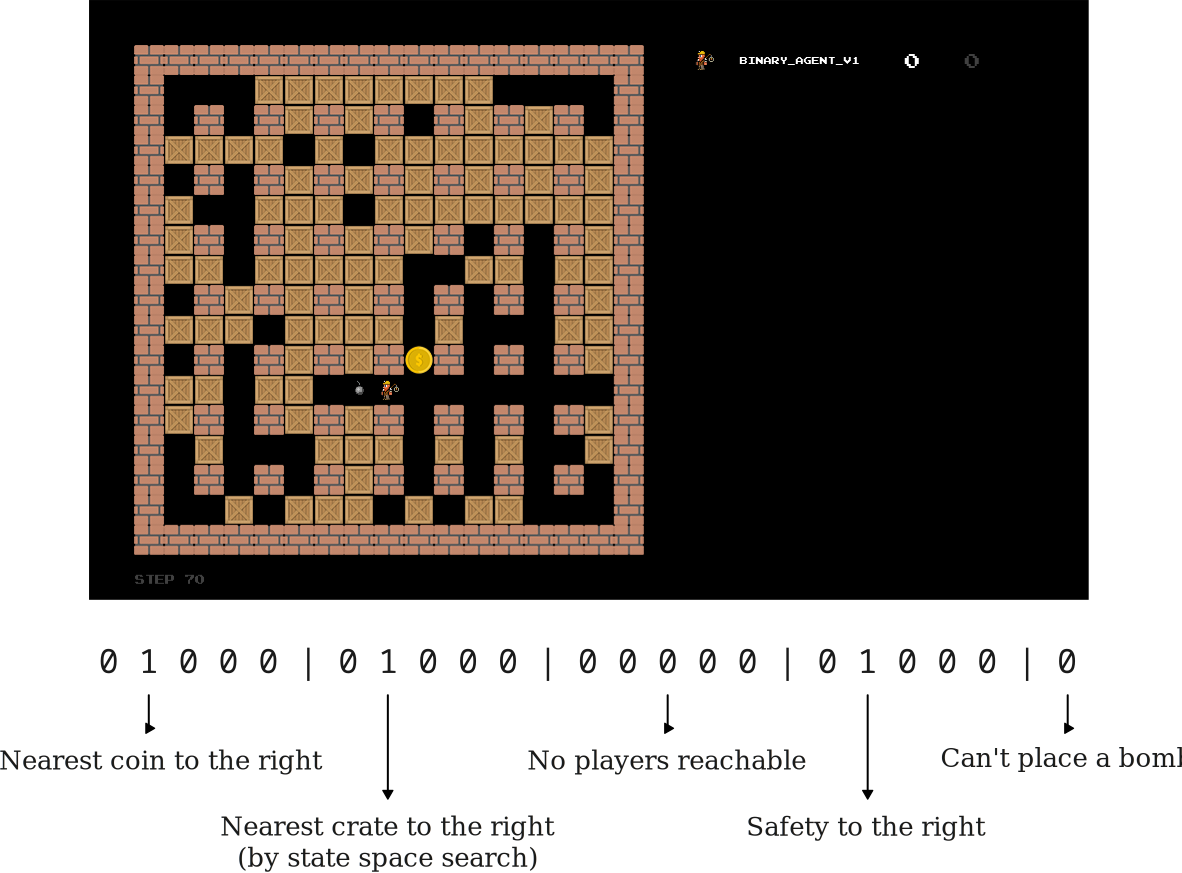
\includegraphics[width=.8\linewidth]{figures/q-vector.pdf}
    \caption{Sample feature vector corresponding to a state of the game.}
    \label{fig:q-vector}
\end{figure}

\begin{figure}[b]
    \centering
    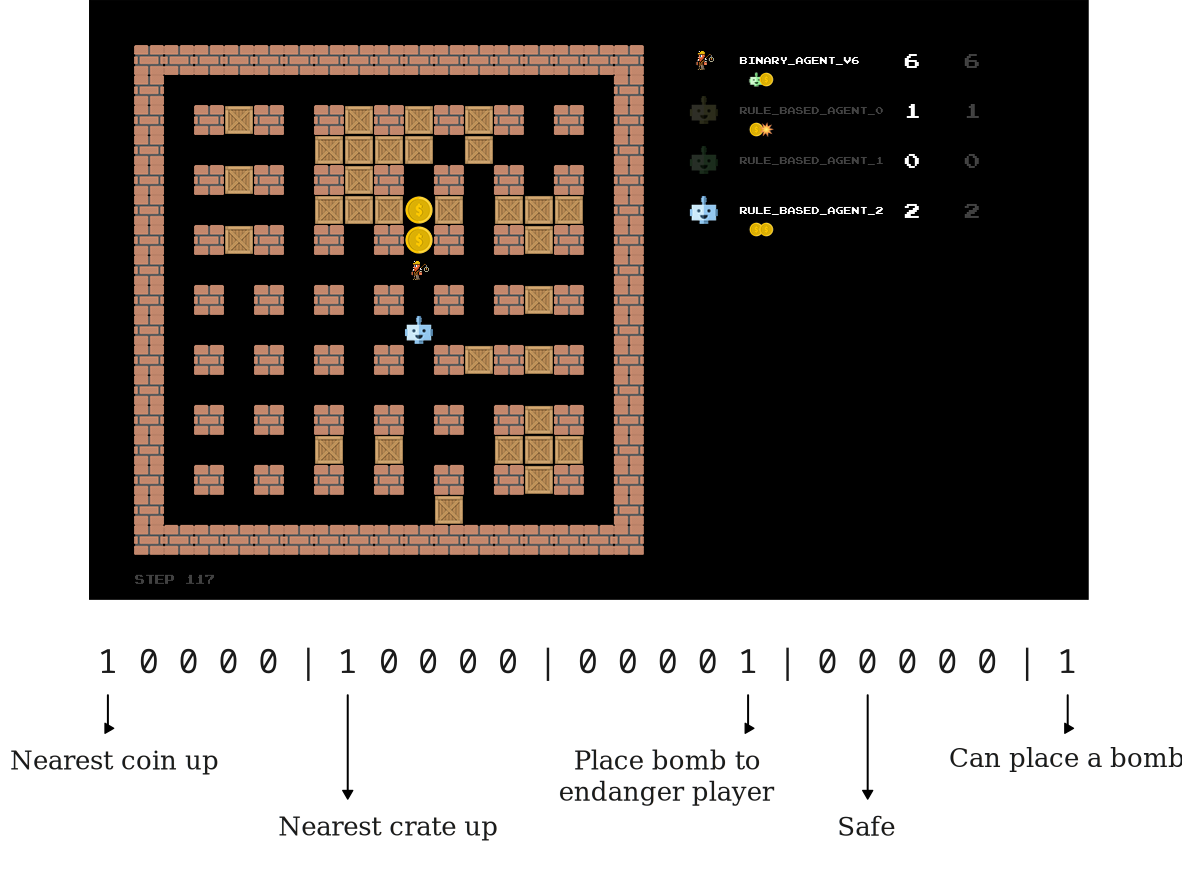
\includegraphics[width=.8\linewidth]{figures/q-vector-2.pdf}
    \caption{Another sample feature vector corresponding to a state of the game.}
    \label{fig:q-vector-2}
\end{figure}

The direction segments are defined as up/right/down/left/wait and, in the case of the direction to where placing a bomb will endanger another player, the wait can be also interpreted as "place a bomb to do so".

All of the features are calculated by searching the state space of the game (assuming that other players stand still), meaning that a path is found even if there are ongoing explosions / crates that will be gone by the time the agent gets to them.
This is almost always desirable as the shortest path on the board is not necessarily the shortest path step-wise.

To make the agent's decision making easier, directions to coins/crates/players are masked by the safety direction vector (if it isn't empty), since it's essentially never useful for the agent to move in such a way that will result in their death.

In cases where the agent is in danger and there doesn't exist a safe state, the directions to safety are instead replaced by directions to a position that is furthest away from the bomb.

We experimented with turning the binary direction vectors into non-binary ones -- if an object is at distance $d$, the value of the direction to it was set to $1/d$.
Note that this differs from the distance agent, since here we only have the distance to the closest target, instead of checking the distance in each direction.
The best trained agent with this approach was only slightly weaker than the best binary agent (but wasn't trained for as long due to time constraints).

The method was implemented via PyTorch \cite{pytorch}, taking heavy inspiration from PyTorch's sample implementation of DQN \cite{pydqn}.
The network itself is implemented using $n$ hidden linear layers, using ReLU as the activation function.

\clearpage

\subsubsection[Distance features]{Distance features {\normalsize \normalfont \it \hfill Jannis}}

This approach differs from the previous one mostly in feature selection: Instead of binary features signaling the preferable direction, the agent is told the distance to the closest coin, crate, enemy and safe position (provided the agent is in danger) in each direction. More precisely, the feature vector contains the following values:

\begin{itemize}
    \item positions $\phantom{0}1 \ldots \phantom{0}5$: distance to the nearest \textbf{coin} in each direction
    \item positions $\phantom{0}6 \ldots 10$: distance to the nearest \textbf{crate} in each direction
    \item positions $11 \ldots 15$: distance to the nearest position where placing a bomb will \textbf{endanger a player}
    \item positions $16 \ldots 20$: distance to \textbf{safety} in each direction (if in danger of dying)
    \item position\phantom{s} $21$: \textbf{can place a bomb} and there is a way to escape it
\end{itemize}

An example of this can be seen in Figure~\ref{fig:distance-vector}. Observe that, due to our implementation of the path-finding algorithm, the agent can observe the revealed coin through the ongoing explosion only because it is safe to pursue it immediately; the explosion will be gone in the next time step. The fifth entry in each set is still a binary feature indicating if the agent is in the optimal spot, for example standing next to a crate.\par

\begin{figure}[h]
    \centering
    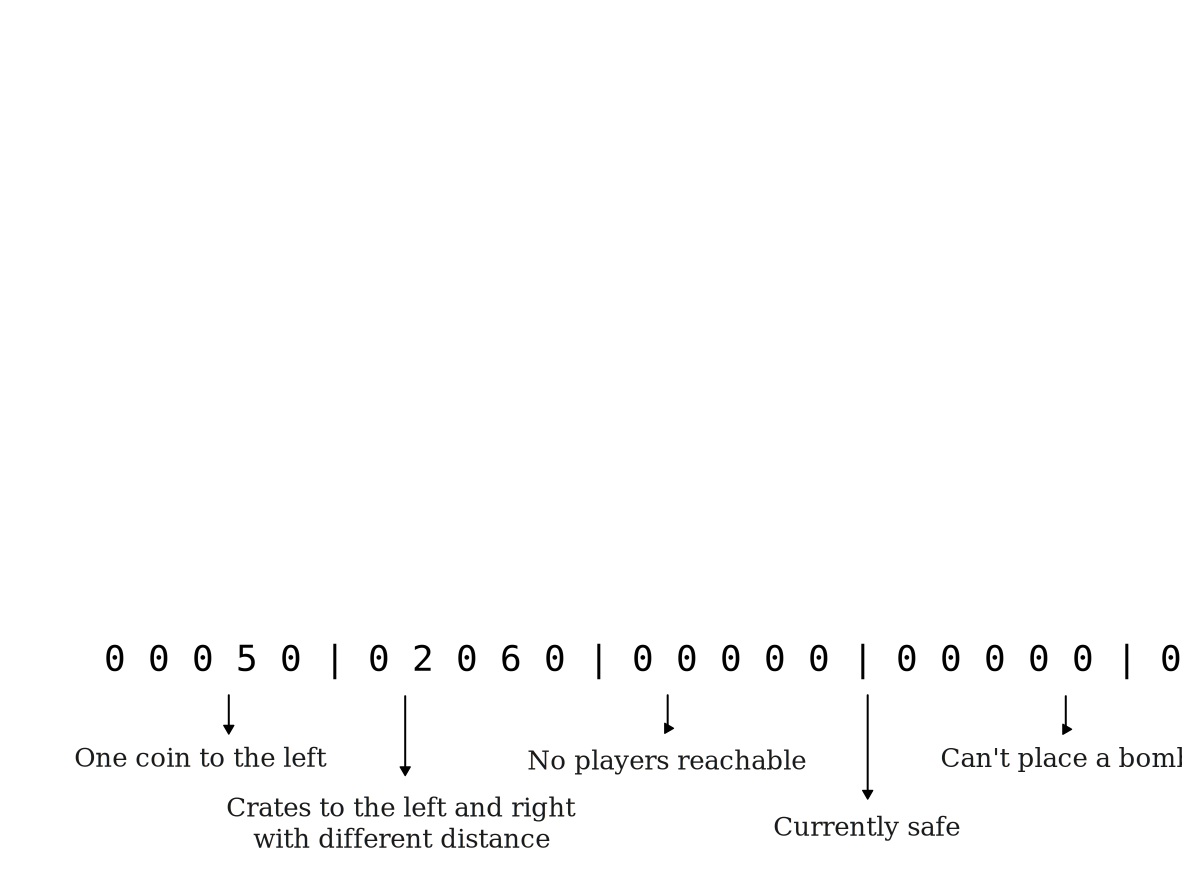
\includegraphics[width=.8\linewidth]{figures/distance-vector.png}
    \caption{Sample distance feature vector corresponding to a state near the start of the game. The agent can weigh the significance of blowing up a nearby crate and collecting a more distant coin, and it chooses the latter.}
    \label{fig:distance-vector}
\end{figure}

Because the binary features are fully constructable from these distance features, the agent is receiving strictly more information.

There are two more changes from the binary agent: Firstly, features are not masked when in the explosion radius of a bomb, so the agent has to learn to heavily prioritize the features relating to danger, and secondly, it uses a softmax policy instead of a greedy one in an attempt to forego infinite behavior loops\footnote{Both versions use $\epsilon$-exploration during training.}.

\clearpage

\section[Training]{Training {\normalsize \normalfont \it \hfill Tomáš}}

For training the agents, we developed a number of utility scripts to simplify the process of training.

The first is \texttt{train.py}, which defines a number of subcommands (called 'tasks') for training the agent to perform specific things.
It comes with useful flags like \texttt{--infinite <n>}, which repeats the last $n$ commands indefinitely and \texttt{--continue}, which continues the training process instead of resetting the model.

As an example, the task \texttt{"complete"} fully trains the agent by running the following subcommands:
\begin{minted}{python}
TASKS = {
    ...
    "complete": [
        # first learn to pick up coins
        (["--scenario", "coin-heaven", "--n-rounds", "100"], False),
        # then learn to hunt/evade the rule-based agent
        (["rule_based_agent", "--scenario", "empty", "--n-rounds", "1000"], False),
        # then learn to work with crates
        (["--scenario", "classic", "--n-rounds", "1000"], False),
        # then learn to work with crates + hard agent
        (["rule_based_agent", "--scenario", "classic", "--n-rounds", "200"], True),
        # then learn to work with crates + really hard agent
        (["binary_agent_v3", "--scenario", "classic", "--n-rounds", "200"], True),
        # finally play against itself (None gets substituted)
        ([None, "--scenario", "classic", "--n-rounds", "200"], True),
    ],
    ...
}
\end{minted}

The boolean value in the tuple indicates whether the elo of the agent should be calculated using the \texttt{elo.py} utility script, which simulates a specified number of games of the agent against those already in the database and then outputs the elo.
This, while slowing down the training process, is vital for determining whether the agent's performance is improving.

\subsection[\texttt{q\_agent}]{\texttt{q\_agent}{\normalsize \normalfont \it \hfill Behrooz}}

The process of training different versions of q-agent, \textit{the agent that is completely based on lookup table}, works on the Bellman function and various utility scripts that was designed to let the agent to explore the field, discover the new states and learn the best action in the corresponding state.

\subsubsection[Exploration vs. Exploitation]{Exploration vs. Exploitation{\normalsize \normalfont \it \hfill Behrooz}}

As mentioned in the \textit{Methods} section, subsection of \textit{Q-table}, according to the number of features, two different techniques of implementation was employed. In the very first version of q-agent the whole world was given to the agent, whereas in the other versions it was the responsibility of the agent to explore the world. This approach is called \textit{Model free reinforcement learning}\cite{INTUITIVE-REINFORCEMENT}, in which the agent simultaneously learns the policy and implicitly world behavior. At this point the trade off between exploration, \textit{learning more about the world}, and exploitation, \textit{fine tuning the current policy and maximizing the reward, in other words staying in the comfort zone} happens. To lead the agent in the right direction of learning, a reward system and utility scripts were used. The significant issue of this method is local maximas or \textit{local minimas, not applicable in this game}, where the agent will not leave its comfort zone. Fine tuning of the rewards as well as hyperparameters are the most time consuming part of training. In the following the whole process of this trade off is illustrated.

\textbf{\textit{Initialize Q-table}}

As it was explained the q-agent comprehends each state by traveling across the field, therefore each new action in that state would have been initialized by the Q-value of equal to zero.

\begin{minted}{python}
# if the state is new, add it to the Q-table and initialize the table with zero value 
if self.model.get(state) is None:
    self.model[state]= dict.fromkeys(ACTIONS, ZERO)
\end{minted}

\textbf{\textit{Game rewards}}


To guide the agent an accurate system of rewards should be planned, in which the agent learns immediately the result of its action and not the result of beforehand actions that might have happened in some other states (and) or in the past but the consequence is showing off now. Therefore a reward system based on \textit{immediate consequence} was employed. For instance, instead of using the event \texttt{BOMB\_EXPLODED}, the event \texttt{PLACED\_USEFUL\_BOMB} or \texttt{PLACED\_SUPER\_USEFUL\_BOMB} were used, where the action is valuated based on current action of the agent not the one that was occurred between 1-3 steps ago. Moreover, it was tried that symmetric events such as both \texttt{DID\_NOT\_MOVED\_TOWARD\_CRATE} and \texttt{MOVED\_TOWARD\_CRATE} in the system rewards to be employed to accelerate the process of learning. It happened during the game playing that the agent did not know what to do with different nearest items. The finalized reward system is as follow for \texttt{q\_agent} version II which focused on extracting the maximum available states in various scenarios to exploit this information for further training:  

\begin{minted}{python}
GAME_REWARDS = {
    # hunt coins
    MOVED_TOWARD_COIN:50,
    DID_NOT_MOVE_TOWARD_COIN: -25,
    e.COIN_COLLECTED: 300,

    # hunt people
    MOVED_TOWARD_PLAYER: 1,

    # blow up crates
    MOVED_TOWARD_CRATE: 50,
    DID_NOT_MOVE_TOWARD_CRATE: -80,

    # basic stuff
    e.INVALID_ACTION: -500,
    DID_NOT_MOVE_TOWARD_SAFETY: -1000,
    MOVED_TOWARD_SAFETY: 800,

    # be active!
    USELESS_WAIT: -200,

    # meaningful bombs
    PLACED_USEFUL_BOMB: 350,
    PLACED_SUPER_USEFUL_BOMB: 500,
    DID_NOT_PLACE_USEFUL_BOMB: -600,
}
\end{minted}

To find the best value for each event and tuning the agent's actions, many different training sessions ran. Any misappropriate change to the system led the agent to one of the many local maximas in the games. To avoid this, a fixed randomness of three percent was employed in choosing the actions during playing mode to release the agent from any probable local maximas. During playing mode the agent must choose the best action according to the corresponding state from the pre-learned actions, and if it is a new state which has not been yet encountered, it must choose a complete random action.

\textbf{\textit{Utility scripts}}

To encounter the maximum states and regarding best action in that state, the agent has been trained with different scenarios, fields and number of rounds as well as against variant opponents. In the following extraction code the process of training \texttt{q\_agent} version II is clearly presented:

\begin{minted}{python}
# Different scenarios to learn the world
tasks = {
    "1": [
        f"--no-gui --agents {arguments.training_agent} 
                                --scenario coin-heaven --n-rounds 5000",
        
        f"--no-gui --agents {arguments.training_agent} 
                                --scenario sparse-crate --n-rounds 30000",
        
        f"--no-gui --agents {arguments.training_agent} peaceful_agent 
                                --scenario sparse-crate --n-rounds 40000",
                                
        f"--no-gui --agents {arguments.training_agent} peaceful_agent 
                                --scenario classic --n-rounds 40000",
                                
        f"--no-gui --agents {arguments.training_agent} peaceful_agent 
                                rule_based_agent --scenario classic 
                                --n-rounds 40000",
                                
        f"--no-gui --agents {arguments.training_agent} rule_based_agent 
                                rule_based_agent rule_based_agent 
                                --scenario classic --n-rounds 100000"

    ]
}
\end{minted}

To make the affect of each training scenario intelligible, the following can be added that in:


\begin{enumerate}
    \item coin-heaven scenario it learns how to collect the coins and encounters all possible states in 5000 rounds,
    \item sparse-crate scenario it learns how to destroy crates and run to safety with random placement of crates to encounter most probable different placement of crates in 30000 rounds,
    \item sparse-crate scenario against peaceful agent it learns how to differentiate the \texttt{PLACED\_USEFUL\_BOMB} and \texttt{PLACED\_SUPER\_USEFUL\_BOMB}, which will destroy the \textit{crates} and \textit{crates and enemy} respectively in 40000 rounds
    \item classic scenario it learns to encounter the real states regarding the competition condition in 40000 rounds
    \item classic scenario it will face an agent that can kill it, therefore, escaping from the others' bomb is learned here
    \item classic scenario it encounters the real game condition with all the possibilities of events and experiences them in one hundred thousand rounds
\end{enumerate}


The remarkable fact about the number of states that the agent encounters was that in the coin-heaven scenario after 5000 rounds of game, there were just about 100 states stored in the Q-table and if 10000 rounds were played barely new state would be added. Therefore, the number of rounds that the agent should be trained in each scenario comes from a lot of experiments. 


This process of learning was implemented in \texttt{train\_q.py} file.

\subsubsection[Bellman equation]{Bellman equation{\normalsize \normalfont \it \hfill Behrooz}}

The Bellman equation in this game had some conditions that lead variant implementation of it according to each condition. Generally the Q-value was updated by using the following implemented Bellman function code:

\begin{minted}{python}
# if action is valid, update the Q_value of that state_action
elif (self.model[state][action] is not None) and new_state: 

    model_new_result = self.model[new_state]
    max_result = max(model_new_result.values())

    self.model[state][action] = self.model[state][action] + LEARNING_RATE * \
        (reward + GAMMA * max_result - self.model[state][action])
\end{minted}

There were invalid actions such as crossing walls, picking bomb, etc., that the agent should not do. Therefore, the agent was penalized for that actions, to find out to what extend should the agent be penalize, various approaches was tested during the training from zero value to minus infinity, however, the best one came from \texttt{EVENTS}, namely \texttt{INVALID\_ACTION}. Nevertheless, tuning the value of this event took a great deal of hours.

 \begin{minted}{python}
# invalid action then penalize the agent with invalid action
if new_state is None or self.model.get(new_state) is None: 
    self.model[state][action] = self.model[state][action] + ( 
    LEARNING_RATE * (reward + GAMMA * 
    (GAME_REWARDS[e.INVALID_ACTION]) - self.model[state][action]))
 \end{minted}

\subsubsection[Epsilon greedy policy]{Epsilon greedy policy{\normalsize \normalfont \it \hfill Behrooz}}

Learning process is extremely time consuming for both the agent and the designers of the agent. Adjusting the hyperparameters is one of those.

\textbf{\textit{Hyperparameters}}

\begin{minted}{python}
# Training parameters
LEARNING_RATE = 0.9

# Environment parameters
GAMMA = 0.99

# Exploration parameters
MAX_EPSILON = 1 
MIN_EPSILON = 0.1 
DECAY_RATE =  0.0001
\end{minted}

By such hyperparameters, which will lead the \texttt{q\_agent} version II to explore the field as much as it can, the game starts at maximum randomness of one hundred percent and very slowly decrease until ten percent at 30000th round of the game. Afterwards the agent would play mostly based on its previous experience of the game. This setting will provide the opportunity of discovering the most states in the game in order to be prepared for the real game. Therefore, the agent will encounter the least possible unknown states during the real game. However, it is pointless if the randomness is avoided during the real game. This avoidance will lead the agent to local maxima instead of global one. The amount of randomness is calculated for each step in the game by following code:

\begin{minted}{python}
epsilon = MIN_EPSILON + (MAX_EPSILON - MIN_EPSILON) * \
    np.exp(-DECAY_RATE * game_state['step'])
\end{minted}

With a Probability of $1 - \varepsilon$, agent does exploitation, and with the probability $\varepsilon$, it will do exploration.
acting based on epsilon greedy policy has the following steps:

\begin{enumerate}
    \item Generate the random number between 0 to 1.
    \item If the random number is greater than epsilon, do exploitation.take the action with the highest value given a state.
    \item Else, do exploration (Taking random action).
\end{enumerate}



\begin{minted}{python}
def _epsilon_greedy_policy( model: dict, state: list,  epsilon: float) -> str:
    random_int = random.uniform(0,1)
    if state and random_int > epsilon:
        action = _greedy_policy(model,state)
    else:
        action = random.choice(ACTIONS)
    return action
\end{minted}

Q-learning is an off-policy algorithm which means that the policy of taking action and updating function is different.
In bomberman game, the Epsilon Greedy policy is acting policy, and the Greedy policy is updating policy.
The Greedy policy will also be the final policy when the agent is trained. It is used to select the highest state and action value from the Q-Table.

\begin{minted}{python}
def _greedy_policy(model: dict, state: list) -> str:
    state = tuple(state)
    action = np.argmax(model[state])
    action = ACTIONS[action]
    return action
\end{minted}


\subsubsection[Choosing action]{Choosing action{\normalsize \normalfont \it \hfill Behrooz}}

choosing the action from the Q-table at a very early step of the training will cause limited perspective view of the game. Therefore, random action was added to the game at every stage of it that was necessary. In the following cases, randomness will help the agent to choose an action:

\textbf{\textit{Random actions}}

\begin{enumerate}
    \item if the state is unknown, \textit{\texttt{[9]th} comment in code}
    \item during the play mode, \textit{\texttt{[7]},fixed amount of 3 percent}
    \item If there is more than one best action, used for new encountered states with all zero values, \textit{\texttt{[6]}}
    \item during the train mode, \textit{\texttt{[3]}, at a decreasing rate}
\end{enumerate}

Otherwise the action will be chosen from the pre-learned action-state pairs from the Q-table.

The following is the whole process of choosing action in different conditions that the agent will encounter.

\begin{minted}{python}
# [1] If the encountered state has values in it for the actions
if model_result.values() is not None: 
    # [2] Choose a random number between one and zero 
    random_int = random.uniform(0,1)
    # [3] If in training MODE
    if self.train:
        # [4] Calculation of epsilon
        epsilon = MIN_EPSILON + (MAX_EPSILON - MIN_EPSILON) 
                    * np.exp(-DECAY_RATE * game_state['step'])
        # [5] Go for random action at a decreasing percentage of randomness
        if random_int <= epsilon: 
            action = random.choice(ACTIONS)# without bomb
            return action
        # [6] Choose from the Q_Table the best action that is stored,
        #if more than one best action, choose one randomly
        # useful for new states that have been just initialized
        max_value = max(model_result.values())
        possible_actions = 
            [key for key, val in model_result.items() if abs(max_value - val) < 1e-4]
        action = random.choice(possible_actions)
        return action
    # [7] Having a fixed randomness even if there is best action 
    epsilon = .03
    if random_int <= epsilon:
        action = random.choice(ACTIONS)
        return action
    # [8] Choosing from Q_Table
    action = np.argmax(list(model_result.values()))
    action = ACTIONS[action]
    return action
# [9] if the encountered state is unknown to the agent, add it to the Q-table
else:
    action = random.choice(ACTIONS)
    self.model[state]= dict.fromkeys(ACTIONS, ZERO)
    return action
\end{minted}

\subsubsection[Hyperparameter improvements]{Hyperparameter improvements{\normalsize \normalfont \it \hfill Jannis}}

Late into the development process, we decided to revisit the Q-table method with the knowledge gained in our neural network endeavors. Firstly, we replaced the auxiliary rewards with those that worked well for \texttt{binary\_agent}:

\begin{minted}{python}
GAME_REWARDS = {
    # hunt coins
    MOVED_TOWARD_COIN: 50,
    DID_NOT_MOVE_TOWARD_COIN: -100,

    # hunt people
    MOVED_TOWARD_PLAYER: 25,
    DID_NOT_MOVE_TOWARD_PLAYER: -10,

    # blow up crates
    MOVED_TOWARD_CRATE: 1,

    # basic stuff
    e.INVALID_ACTION: -100,
    DID_NOT_MOVE_TOWARD_SAFETY: -500,

    # be active!
    USELESS_WAIT: -100,

    # meaningful bombs
    PLACED_USEFUL_BOMB: 50,
    PLACED_SUPER_USEFUL_BOMB: 150,
    DID_NOT_PLACE_USEFUL_BOMB: -500,
}
\end{minted}

These rewards seemed overall more balanced and less prone to unwanted behavior; for example, by the previously chosen values, the agent is rewarded for placing a useless bomb and subsequently running away from it.\par
Secondly, we decreased the exploration parameter and increased its decay:

\begin{minted}{python}
MAX_EPSILON = 0.1
MIN_EPSILON = 0.0
DECAY_RATE =  0.01
\end{minted}

After only an hour of training with the \texttt{"q-table"} task, the resulting agent dominated its previous versions and stood somewhat of a fighting chance against \texttt{rule\_based\_agent}, as shown in Figure~\ref{fig:q_agent_v3_performance}. With more fine-tuning and longer training, it might have caught up to the neural network methods, alas we did not have time for it.

\begin{figure}[h]
    \centering
    \includegraphics[width=.7\linewidth]{figures/q_agent_v3_performance.png}
    \caption{Results of 100-round duels between the improved agent (\texttt{q\_agent\_v3}) and its predecessors as well as \texttt{rule\_based\_agent}.}
    \label{fig:q_agent_v3_performance}
\end{figure}

\clearpage

\subsection[\texttt{binary\_agent}]{\texttt{binary\_agent}{\normalsize \normalfont \it \hfill Tomáš}}

The training of the different versions of the binary agent was done in the following way:
\begin{enumerate}
    \item run \texttt{train.py} with the \texttt{"complete"} task and \texttt{--infinite 2} to repeat the last 2 commands
    \item manually pick the best-performing model out of the ones where elo was calculated
    \item decrease \texttt{EPS\_START}, \texttt{EPS\_END}, \texttt{TAU} and \texttt{LR} hyperparameters (see next section) for finer convergence
    \item go to step 1 (and use \texttt{--continue} to not overwrite the model)
\end{enumerate}

Besides this, the versions also differ by minor bugfixes, optimizations and refactors.
These are however limited and don't change the structure of the network, meaning that the training doesn't need to be restarted.

\subsubsection[Hyperparameters]{Hyperparameters {\normalsize \normalfont \it \hfill Tomáš}}

For training the network, the following hyperparameters are available:

\begin{minted}{python}
BATCH_SIZE = 256    # number of transitions sampled from replay buffer
MEMORY_SIZE = 1000  # number of transitions to keep in the replay buffer
GAMMA = 0.99        # discount factor (for rewards in future states)
EPS_START = 0.10    # starting value of epsilon (% for taking random actions)
EPS_END = 0.05      # ending value of epsilon
EPS_DECAY = 10      # how many _steps_ (not rounds) until full decay
TAU = 1e-3          # (soft) update rate of the target network
LR = 1e-4           # learning rate of the optimizer
OPTIMIZER = optim.Adam      # the optimizer
LAYER_SIZES = [1024, 1024]  # sizes of hidden layers
\end{minted}

All of these were heavily experimented with and the following values were found out to work best for the task.
This section discusses the more important ones, since some didn't seem to affect the training too much.

The training utilizes epsilon decay to start the agent off with making random moves with a change \texttt{EPS\_START}, which get gradually less probable in \texttt{EPS\_DECAY} steps, all the way to \texttt{EPS\_END}.
This is counter to the usual approach which decays over games and not rounds, but we found that per-round decay has a faster convergence.
This could possibly be explained by the fact that the agent has to do a number of essentially determined moves at the start to get out of the small starting area and randomizing more at the start allows it to do that.

The network contains hidden layers of sizes $(1024, 1024)$, which is a large enough number of neurons to handle the task at hand efficiently.
Selecting a lower number (eg. one / two layers of size $128$) was attempted and the agent initially learned well, but would eventually get stuck in bad local optima, which suggested to us that a larger network was necessary.
Conversely, using a larger network seemed to have no visible benefits and only decreased the speed at which the agent learned.

\subsubsection[Events]{Events {\normalsize \normalfont \it \hfill Tomáš}}

The binary agent defines the following custom events:

\begin{minted}{python}
# movement events
MOVED_TOWARD_COIN / DID_NOT_MOVE_TOWARD_COIN
MOVED_TOWARD_CRATE / DID_NOT_MOVE_TOWARD_CRATE
MOVED_TOWARD_SAFETY / DID_NOT_MOVE_TOWARD_SAFETY
MOVED_TOWARD_PLAYER / DID_NOT_MOVE_TOWARD_PLAYER

# bomb events
PLACED_USEFUL_BOMB  # will destroy crate
PLACED_SUPER_USEFUL_BOMB  # endangers opponent
DID_NOT_PLACE_USEFUL_BOMB  # does nothing

# sent when a movement action could have been made but the agent waited
USELESS_WAIT   
\end{minted}

The best version of the agent was trained using the following set of events:

\begin{minted}{python}
GAME_REWARDS = {
    # hunt coins
    MOVED_TOWARD_COIN: 50,
    DID_NOT_MOVE_TOWARD_COIN: -100,

    # hunt people
    MOVED_TOWARD_PLAYER: 25,
    DID_NOT_MOVE_TOWARD_PLAYER: -10,

    # blow up crates
    MOVED_TOWARD_CRATE: 1,

    # basic stuff
    e.INVALID_ACTION: -100,
    DID_NOT_MOVE_TOWARD_SAFETY: -500,

    # be active!
    USELESS_WAIT: -100,

    # meaningful bombs
    PLACED_USEFUL_BOMB: 50,
    PLACED_SUPER_USEFUL_BOMB: 150,
    DID_NOT_PLACE_USEFUL_BOMB: -500,
}
\end{minted}

The agent noticeably doesn't take advantage of events such as \texttt{OPPONENT\_ELIMINATED}, \texttt{CRATE\_DESTROYED}, and other seemingly useful ones.
This is because to use them, the training would have to reward states sufficiently far into the future (in our case based on time to detonate a bomb), otherwise the agent associates the high positive/negative reward with the wrong action.
Since the training code by default receives a (current state, action, next state, events) tuple, it is much simpler (but arguably not as clean) to only restrict the events to those with immediate rewards.

The event values were picked in such a way that the agent prefers picking up coins, then hunt players and lastly blows up crates, which seems to work well against the base agents.
They are also selected to prevent looping, which was an issue for earlier versions of the agent, where it would oscillate back and forth because sum of the rewards was positive (which can't occur here).

\clearpage

\subsection[\texttt{distance\_agent}]{\texttt{distance\_agent}{\normalsize \normalfont \it \hfill Jannis}}

The training of the neural-network agent with distance features used the same utility scripts and generally followed the same methodology of the version with binary features. Because the binary agent seemed to outperform the distance agent in early testing, more effort was put toward training the binary version.

\subsubsection[Hyperparameters]{Hyperparameters{\normalsize \normalfont \it \hfill Jannis}}

The network employs hyperparameters similar to its binary counterpart:

\begin{minted}{python}
BATCH_SIZE = 256    # number of transitions sampled from replay buffer
MEMORY_SIZE = 3000  # number of transitions to keep in the replay buffer
GAMMA = 0.99        # discount factor (for rewards in future states)
EPS_START = 0.1     # starting value of epsilon (for taking random actions)
EPS_END = 0.01      # ending value of epsilon
EPS_DECAY = 100     # how many rounds until full epsilon decay
TAU = 1e-3          # update rate of the target network
LR = 1e-4           # learning rate of the optimizer
OPTIMIZER = optim.Adam                # the optimizer
LAYER_SIZES = [500, 2000, 2000, 500]  # sizes of hidden layers
\end{minted}

The two major changes are the use of a larger network due to more complex features and the fact that the exploration measure $\epsilon$ depends on the number of rounds instead of the number of steps. Additionally, the memory size was increased. Due to time constraints, all of these changes were not tested rigorously enough to conclude the superiority of one approach over another.

\clearpage

\section[Experiments and Results]{Experiments and Results{\normalsize \normalfont \it \hfill Tomáš}}

The overall performance of the implemented agents is shown in figure \ref{fig:elos}.

\begin{figure}[h]
    \centering
    \includegraphics[width=\linewidth]{figures/elo.pdf}
    \caption{Elo ratings (with standard deviation) of the implemented agents.}
    \label{fig:elos}
\end{figure}

The first four agents are some of the built-in agents that the repository contained.
The \texttt{coin\_collector\_agent} and the \texttt{rule\_based\_agent} are the strongest ones out of those, having relatively advanced logic for collecting coins and preventing being killed by explosions, so they are the ones the agents aim to beat.
The \texttt{peaceful\_agent} and \texttt{random\_agent} are, as the name and elo suggests, mostly a sanity check (since they don't really do anything) and thus should never win against our agents.

As we can see, the strongest agent is the last binary agent, followed by the distance one and lastly the Q-agent, whose performance is the weakest.
The following subsections discuss each of these in turn.


\clearpage

\subsection[\texttt{q\_agent}]{\texttt{q\_agent}{\normalsize \normalfont \it \hfill Behrooz}}
% headings are always plain text (so it's bold and doesn't look weird in the table of contents)


The following table shows the different scenarios that the agent was trained with. Some interesting fact about the this simple approach, \textit{lookup table}, is as follows:

\begin{itemize}
    \item Number of rounds to discover the maximum states at maximum randomness would not exceed of 220,000 
   \item The maximum number of encountered state is far away from the theoretical calculation.
    \item The running time of the algorithm is short regarding the amount of randomness that is used.
\end{itemize}

\begin{figure}[h]
    \centering
    \includegraphics[width=0.9\linewidth]{figures/q-table/q-agent-table.pdf}
    \caption{Experiment of the different scenarios in training the q-agent. The numbers are approximately regarding the randomness that is used in training. However, this approximation arises from more than 600 hours of training.}
    \label{fig:q-agent-table}
\end{figure}

As it is clear from training of the agent against the same agent but different field or even training the agent with the same scenarios, \textit{doubled run}, neither add new states to the Q-table nor improve the performance of the agent. 

Compared to other methods of implementing the bomberman game, in Q-table approach, the agent should be trained in the real scenarios that it is supposed to play after training. As it is evident in the table, the most states of the game has been learned during the real scenario, \textit{classic with 3 opponents in this competition}. However, this exploration will not lead the agent to face new states after some rounds, \textit{overall 220,000 rounds}. At this point tuning the hyperparameters and values of rewards will help the agent to improve its performance. Nevertheless, this improvement is not remarkable. After train in each scenario the agent is able to play that scenario with a reasonable rate of success, but when new Q-values are added to the Q-table or the previous Q-values are updated the performance of the agent would negatively be affected, which shows instability of agent in different scenarios. Moreover, if the agent is trained in more number of rounds that it should be, the agent would got stuck in one of many local maximas in the game.

Q-table approach is simple but needs too much consideration to be able to compete against other agents. It is very sensitive to any change in hyperparameters or reward system. The process of training is complicated and too hard to make the agent act robustly. Therefore, using another techniques such as Deep Q-Network is suggested, which is explained in this report and corresponding results are clearly defining the differences.

\clearpage

\subsection[\texttt{binary\_agent}]{\texttt{binary\_agent}}

\subsubsection[Optimizations]{Optimizations {\normalsize \normalfont \it \hfill Tomáš}}

The bulk of writing the binary agent code included optimizations, since searching the state space for crates, coins, enemies and safety is a non-trivial computation -- having to simulate things like explosion maps and crate updates takes time.

The first version of the agent code created new game state copies via \texttt{copy.deepcopy}.
This is simple and straightforward but very slow, since the entire game state is copied, even if we were to only change a portion.
This is why the \texttt{copy.copy} function is a better choice, with the code creating new instances of lists/arrays only when strictly necessary.

Another major optimization is LRU caching of certain functions.
One of the obvious candidates is the \texttt{get\_blast\_coords} function, which returns blast coordinates of a bomb with a given position -- since these never change, no matter the game state, it can be safely cached once calculated.
Another, less obvious one, is the \texttt{state\_to\_features} function itself (for training) -- since we're receiving \texttt{(old\_state, new\_state)} pairs, the hit rate will be at least 50\% due to the overlap, which is definitely worth caching.

To show that these improvements are quite substantial, the agent was profiled on 10 rounds of the coin-heaven scenario with and without caching / copying.
The results can be seen in figure \ref{fig:optimization} -- as we can see, both optimizations drastically improve the speed of the training.
Not using \texttt{copy.deepcopy} leads to over a $10 \times$ improvement, with a further improvement of over $2 \times$ due to caching (as suggested in the previous paragraph).

\begin{figure}[h]
    \centering
    \includegraphics[width=1\linewidth]{figures/optimization.pdf}
    \caption{Runtimes of 10 rounds of coin-heaven training of the binary agent.}
    \label{fig:optimization}
\end{figure}

Although the current runtime of the agent is acceptable for our purposes, the majority of the compute time is still being spent calculating next states on the CPU (over 80\%).
It would be interesting to explore how to put more load on the GPU, since it's currently not fully utilized (although this particular task of state space exploration doesn't suit the GPU too well so this might be difficult).

\newpage

\subsubsection[Learning Plots]{Learning Plots {\normalsize \normalfont \it \hfill Tomáš}}

Since there is too many plots from training to be shown here, below are a few selected ones from subcommands that show the agent learning a number of specific traits.

The first plot \ref{fig:coins} shows the training progress of the binary agent on 100 rounds of coin-haven.
As we can see, the agent learns to successfully complete the first task in approximately 15 rounds, with the rest of the rounds seeing no significant improvement.

\begin{figure}[h]
    \centering
    \includegraphics[width=.8\linewidth]{figures/coins.pdf}
    \caption{Training of binary agent on 100 rounds in the coin-haven scenario. Steps and game score is normalized to have the maximum value of 1 while reward is scaled by an arbitrary number. The initial rounds have a very negative reward whose exact value isn't important.}
    \label{fig:coins}
\end{figure}

The second plot \ref{fig:vs-rule} shows the training progress of the binary agent on 100 rounds of an empty arena against the peaceful agent.
Its purpose is for the agent to learn combat, which consists of moving toward agents, placing bombs that endanger them and running away to safety.
As the plot shows, the agent can solve the second task relatively handily in approximately 30 steps, with the rest of the rounds again showing no significant improvement. 

\begin{figure}[h]
    \centering
    \includegraphics[width=.8\linewidth]{figures/vs-rule.pdf}
    \caption{Training of binary agent on 100 rounds in the empty scenario against a peaceful agent with a sliding window of size 5. Steps and game score is again normalized, with the reward scaled appropriately.}
    \label{fig:vs-rule}
\end{figure}

\clearpage

\subsection[\texttt{distance\_agent}]{\texttt{distance\_agent}}

\subsubsection[Distance vs. inverse distance]{Distance vs. inverse distance{\normalsize \normalfont \it \hfill Jannis}}

Intuitively, things that are close to the agent should be more important than things that are far away. Furthermore, a distance of 1 indicates standing next to something while a distance of 0 implies that nothing could be found in the given direction. In other words, something very important is feature-wise very similar to something unimportant. To help the agent, we tried using inverse distances as features in place of plain distances while leaving 0's unchanged.\footnote{This is implemented as \texttt{binary\_distance\_agent} in the GitHub repository.} For example, the feature vector

\begin{minted}[linenos=false]{python}
0  0  0   5   0 | 0   2   0    6   0 | 0  0  0  0  0 | 0  0  0  0  0 | 0
\end{minted}

would be turned into

\begin{minted}[linenos=false]{python}
0  0  0  0.2  0 | 0  0.5  0  0.17  0 | 0  0  0  0  0 | 0  0  0  0  0 | 0
\end{minted}

Thus, a far-away object looks similar to no object being observed. Somewhat unsurprisingly, this did not significantly change the agent's performance, as it does not fundamentally change the relayed information, and the implemented change can be recreated by a small network.

\subsubsection[Reward shaping]{Reward shaping{\normalsize \normalfont \it \hfill Jannis}}

We tried three approaches:

\textbf{Naïve approach:} In the beginning, we tried to hand-pick auxiliary rewards to gently push the agent's actions in the desired direction. We adhered to the following principles:

\begin{itemize}
    \item Game rewards should generally be larger than auxiliary rewards.
    \item Cycling between states should be detrimental.
    \item Collecting coins should be top priority, with hunting enemies being second and blowing up crates third.
    \item Invalid actions should be heavily punished as they show that the agent does not comprehend the world.
    
\end{itemize}

The following is an example of how we implemented these principles:

\begin{minted}{python}
GAME_REWARDS = {
    # hunt coins
    MOVED_TOWARD_COIN: 4,
    DID_NOT_MOVE_TOWARD_COIN: -6,
    e.COIN_COLLECTED: 10,

    # hunt people
    MOVED_TOWARD_PLAYER: 2,
    DID_NOT_MOVE_TOWARD_PLAYER: -2,
    e.KILLED_OPPONENT: 50,

    # blow up crates
    MOVED_TOWARD_CRATE: 1,
    DID_NOT_MOVE_TOWARD_CRATE: -1,

    # basic stuff
    e.GOT_KILLED: -50,
    e.INVALID_ACTION: -20,
    DID_NOT_MOVE_TOWARD_SAFETY: -10,

    # be active!
    USELESS_WAIT: -1,

    # meaningful bombs
    PLACED_USEFUL_BOMB: 10,
    PLACED_SUPER_USEFUL_BOMB: 20,
    DID_NOT_PLACE_USEFUL_BOMB: -40,
}
\end{minted}

The agent's performance seemed particularly volatile when making small changes in the auxiliary rewards, which made fine-tuning them a sisyphean task. Ultimately, we were unable to train a good agent in this way.

\textbf{Potential-based approach:} Due to the promising theory of potential-based rewards~\cite{potential-reward}, we decided to train the agent with a reward function $F$ of the following type:
\[
F(s, a ,s', r') =  \gamma \cdot \phi(s) - \phi(s'),
\]
where the potential $\phi$ is only dependent on the state, and $\gamma$ is the discount factor. In theory, this should help the agent converge to the optimal policy. In practice, however, it is difficult to design an appropriate potential for the task at hand: If one rewards the presence of a well-placed bomb, then the explosion of that bomb creates a penalty which is independent of the agent's action in the given time step. If, on the other hand, the potential is chosen to be agnostic towards bomb placement, then the agent has a hard time figuring out how to destroy crates. In any case, we could not produce an agent that performed better than random when facing crates.

\textbf{Shoehorn approach:} After observing the success of the ``brute-force" rewards of the binary agent, we decided to test them here as well:

\begin{minted}{python}
GAME_REWARDS = {
    # hunt coins
    MOVED_TOWARD_COIN: 50,
    DID_NOT_MOVE_TOWARD_COIN: -100,

    # hunt people
    MOVED_TOWARD_PLAYER: 25,
    DID_NOT_MOVE_TOWARD_PLAYER: -10,

    # blow up crates
    MOVED_TOWARD_CRATE: 1,

    # basic stuff
    e.INVALID_ACTION: -100,
    DID_NOT_MOVE_TOWARD_SAFETY: -500,

    # be active!
    USELESS_WAIT: -100,

    # meaningful bombs
    PLACED_USEFUL_BOMB: 50,
    PLACED_SUPER_USEFUL_BOMB: 150,
    DID_NOT_PLACE_USEFUL_BOMB: -500,
}
\end{minted}

The initial result was underwhelming; the agent took much longer to learn to collect coins than with the naïve approach, see Figure~\ref{fig:coin_collection_comparison}. However, after a longer training session, the agent soon surpassed its previous iterations. Training was done using the \texttt{"complete"} task explained at the start of this section, i.e. with the following command:

\begin{minted}{python}
python train.py --task complete --infinite 3 --quick distance_agent_v1
\end{minted}

\begin{figure}[h]
    \centering
    \includegraphics[width=.46\linewidth]{figures/coin_collection_naive.png}
    \includegraphics[width=.46\linewidth]{figures/coin_collection_shoehorn.png}
    \caption{Learning comparison between the two approaches in the \texttt{"coin-heaven"} scenario. Step count and game score are normalized. No training takes place in around the first 20 rounds because the replay buffer needs to fill up first. As a side-note, for some reason the agent prefers suicide over collecting the last coin most of the time. We could not adequately explain this phenomenon.}
    \label{fig:coin_collection_comparison}
\end{figure}

The option \texttt{--quick} specifies that after each of the last three training stages (which are cycled due to the option \texttt{--infinite 3}), a duel of 50 rounds between the agent and \texttt{rule\_based\_agent} is performed instead of elo calculation. Figure~\ref{fig:distance_agent_training} shows the result of these duels. The decrease in noise over time is caused by the tweaking of hyperparameters. Specifically, \texttt{EPS\_START} and \texttt{EPS\_END} as well as \texttt{TAU} and \texttt{LR} were lowered over time to arrive at $0.05$, $0$, $10^{-6}$ and $10^{-6}$, respectively. The graph suggests that the agent has mostly reached its peak, but more training might yield a small improvement. Note, however, that the graph displays only a very rough skill metric, as it only shows performance against a single opponent.

\begin{figure}[h]
    \centering
    \includegraphics[width=.6\linewidth]{figures/distance_agent_training.png}
    \caption{The performance of \texttt{distance\_agent\_v1} against \texttt{rule\_based\_agent} over time after the initial three training stages of the \texttt{"complete"} task.}
    \label{fig:distance_agent_training}
\end{figure}

\subsubsection[Comparison to binary agent]{Comparison to binary agent{\normalsize \normalfont \it \hfill Jannis}}

As mentioned before, this agent is receiving strictly more information than the one using binary features. Our hope was that this would lead to a superior agent. Unfortunately, we were unable to surpass the skill level of the binary agent. The issue is most likely trainability: Because the features are more complex, the neural network must learn to recognize more elaborate patterns. This requires a larger network and a more dedicated training procedure. Most of all, it requires more development time, which we did not have.

\clearpage

\subsection[Agent comparison]{Agent comparison {\normalsize \normalfont \it \hfill Tomáš}}

The best-trained agent is the 6th iteration of the \texttt{binary\_agent}.
Its performance in duels in the classic arena against the others is depicted in figure \ref{fig:stacked}, showing that it is beating all of the other agents.

The behavior of the agent is very aggressive -- while it primarily goes after coins, it will always attempt to chase down and kill players if any are reachable.
This works quite well, since the strong base agents (like \texttt{rule\_based\_agent}) are usually focused on placing bombs to blow up crates and thus often end up in dead ends, which the binary agent capitalizes on by placing a bomb they can't escape.

\begin{figure}[h]
    \centering
    \includegraphics[width=1\linewidth]{figures/stacked.pdf}
    \caption{Results of the binary agent (v6) against the other agents in classic arena duels.}
    \label{fig:stacked}
\end{figure}

Two noteworthy agents are peaceful and random, since these always\footnote{There can be certain situations where the agents score some points but this almost never happens since peaceful agent doesn't place bombs (so can't escape) and the random agent usually kills itself pretty quickly.} have a score of 0.
Having a 100\% winrate against them is a good indicator that the agent has reached a state where it no longer accidentally kills itself in the first few rounds of the game, which the weaker ones struggled with.

Although the performance against the default agents is good (\texttt{837:9:154}), it would have been great if the agent won every time.
This is likely impossible, as the \texttt{rule\_based\_agent} contains sufficiently advanced logic to dodge placed bombs and the placement of coins is entirely random (which largely determines the winner), but it is definitely something to strive for.

\clearpage

\section[Conclusion]{Conclusion{\normalsize \normalfont \it \hfill Jannis}}

Using methods from the lecture, we were able to implement and train a strong agent for the Bomberman game in the provided time frame. In light of its outstanding performance against \texttt{rule\_based\_agent}, we feel confident that it is a good contender for the tournament.

\subsection[Current shortcomings]{Current shortcomings{\normalsize \normalfont \it \hfill Tomáš}}

There are still certain cases where the binary agent (our selected one for the competition) is lacking, one of them being that the agent will run away from an explosion when in danger even if it has time to place a bomb.
This was only noticed after the submission deadline and is an unintended consequence of the masking by the safety vector whose wait index gets set to 0 if it can run to safety, making the agent more passive than it should be (although not significantly).

Another is the lack of a feature that could tell the agent "you're in a bad position here if another agent moves this way", as it has no information about the possible future actions of other agents.
Or, more generally, additional features that would allow the agent to calculate how good of a position it is in and move throughout the arena accordingly to not get stuck in corners when enemy players are nearby.
This was something we wanted to implement, but did not find a good way to do so.

\subsection[Possible improvements]{Possible improvements{\normalsize \normalfont \it \hfill Jannis}}

\textbf{n-step TD:} The reward system we used for the final versions of all three methods does not include the two game rewards for picking up coins and killing enemies. Instead, it only relies on adjacent ideas like moving towards coins and good bomb placement. The main reason why simpler approaches fail is that we use one-step TD, which makes it very hard for the agent to understand the causal relationship between bomb placement and its detonation. The obvious solution is to instead implement $n$-step TD, where $n$ is at least as large as the fuse timer. This, together with more straight-forward auxiliary rewards, might free the agent to discover new strategies which went heretofore unrewarded.

\textbf{Prioritized experience replay:} Currently, we are sampling from the experience buffer uniformly at random. To improve on this, one could assign each experience a weight based on how much the expected reward differed from the actual reward. As a result, the agent would likely learn from its mistakes faster.

\textbf{More elaborate training:} Since there are a lot of hyperparameters at play, it would be beneficial to fine-tune each one separately. In particular, the neural network layer sizes were decided after very little testing and went unchanged afterwards.

\textbf{Different features:} Apart from replacing binary features with distance features, we barely experimented with different possibilities for the agent's vision. For instance, it would be interesting to measure how much of an impact the \texttt{"wait"} bits have; perhaps they are more a hindrance than an aid for the \texttt{q\_agent} as they increase the feature space. Moreover, the agent might benefit from a perfect vision of its neighborhood, for example to identify a dangerous dead end in which it might get trapped.


\subsection[Project feedback]{Project feedback{\normalsize \normalfont \it \hfill Tomáš}}

Something that would definitely help out future years' competitors is a better interface for the game state (eg. a class).
This is something we had to implement from scratch (and other competitors will likely have to too, if they want the code to be optimized), but it would be really nice if we could just take a game object and have methods like \texttt{advance\_state(action)} and \texttt{to\_dictionary()}, which would greatly help out with initial prototyping.

Another nice addition would be the game result to game files, since what we currently had to do to calculate the elos is to modify the \texttt{end\_round} function in \texttt{environment.py} to write the resulting agent score to an arbitrary file and then parse the file to calculate the resulting elos.
This is quite inconvenient and it would be nicer if a built-in way (eg. write something to the log file or support a flag that outputs this to \texttt{stdout}) existed to extract this information from played games.

\clearpage

\printbibliography

\vfill
\hfill\begin{minipage}{40em}%
    \Large\it Many thanks to Ullrich Köthe and the tutors behind the Machine Learning Essentials (Summer 2023) for a great lecture and an amazing final project!%
\end{minipage}\hfill
\vspace{8em}

\end{document}